\documentclass[]{article}
\usepackage[dutch]{babel}
\usepackage{graphicx}
%opening
\title{}
\author{Thomas Feys \and Jona Cappelle}

\begin{document}

\maketitle

\tableofcontents


\section{Inleiding}
Ons doel is om de wachtrij in de rabotaria te monitoren. Dit zullen we doen aan de hand van een IR grid sensor (AMG8833). Aan de hand van de uitgelezen waarden zullen we in het tweede semester bepalen hoeveel mensen er in de wachtrij staan. Deze informatie zullen we vervolgens via een app of website verspreiden. 
\section{Sensor}
De sensor die we gebruiken om de wachtrij te monitoren is de AMG8833. Deze IR grid sensor heeft 8x8 pixels die de temperatuur weergeven. Volgens de datasheet kan a.d.h.v. de temperatuur een mens waargenomen worden vanop een afstand van 5 meter. De sensor kan gebruikt worden in 3 verschillende modes: normal, sleep en stand-by. In de normale mode heeft de sensor een verbruik van 4.5 mA. De stand-by mode heeft twee opties; de waardes kunnen geüpdatet worden om de 60 seconden of om de 10 seconden. In deze mode is er een verbruik van 0.8 mA. Als laatste is er de sleep mode deze verbruikt 0.2 mA. Een overzicht van alle modes en de commando's die verstuurd moeten worden om in deze modes te raken wordt weergegeven in figuur \ref{fig:operatingmodes}. Tijdens het testen van de sensor hebben we periodiek geswitched tussen de verschillende power modes. Het resultaat van deze test is te zien in figuur \ref{fig:powertest}. De sensor heeft ook een interrupt pin. Deze pin geneert een interrupt als een van de pixels over of onder een bepaalde waarde gaat. Deze waarde is instelbaar.	
\begin{figure}[!ht]
	\centering
	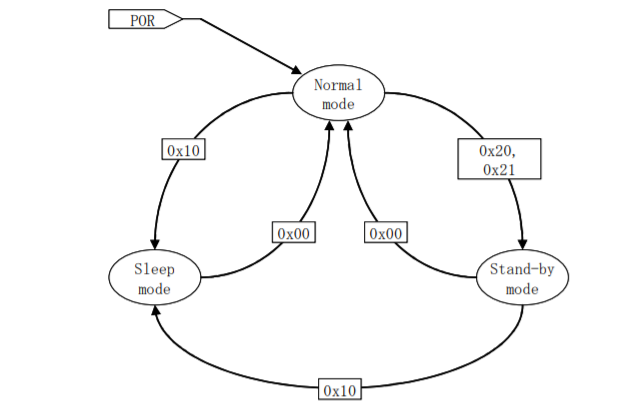
\includegraphics{operatingmodes.png}
	\caption{Overzicht operating modes}
	\label{fig:operatingmodes}
\end{figure}
%todo figuur aanpassen naar screenshot powermodes in de power monitor
\begin{figure}[!ht]
	\centering
	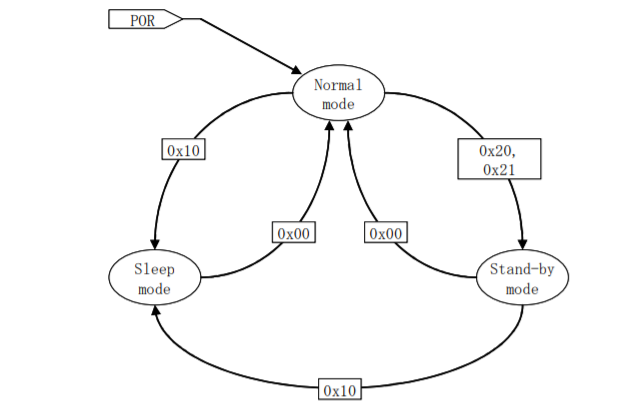
\includegraphics{operatingmodes.png}
	\caption{Test van de verschillende powermodes}
	\label{fig:powertest}
\end{figure}
\section{Systeem}
\subsection{overzicht}
De AMG8833 communiceert met de EFM32 via I2C. Naast de I2C communicatie is er ook een interrupt pin voorzien op de sensor. Deze pin genereert een interrupt als er een van de pixels een bepaalde, instelbare waarde overschrijdt. Een volledig overzicht van het systeem is te zien in figuur \ref{fig:systeem}.
%todo figuur maken in draw.io van het volledige systeem
\begin{figure}[!ht]
	\centering
	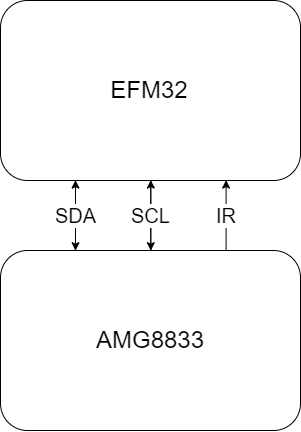
\includegraphics[scale=0.5]{sys.png}
	\caption{Overzicht van het systeem}
	\label{fig:systeem}
\end{figure}
\subsection{I2C}



\section{Code}
\subsection{Functionaliteiten}
Om gemakkelijk met de sensor te werken werd er een library geschreven voor de AMG8833. Er werden verschillende methodes geschreven om vlot te kunnen omgaan met de sensor. Er werd een functie geschreven om alle pixels uit te lezen. Naast de pixels is er ook een thermistor aanwezig in de sensor, ook hiervoor werd een functie geschreven. Er werden ook verschillende functies geschreven om makkelijk tussen de verschillende powermodes te kunnen wisselen. Een volledig overzicht van deze library is te vinden in .....
%todo doxy invoegen en ernaar refereren

\subsection{Flow van de code}
\label{flowcode}
Om het verbruik te minimaliseren wordt er maar om de 5 minuten gecontroleerd of er mensen aanwezig zijn. Omdat de sensor in sleep 0.2 mA verbruikt wordt de sensor volledig uit gezet door de gpio pin uit te zetten. Om de 5 minuten wordt de gpio pin aangezet en de sensor in de stand-by mode gezet waar de waardes om de 60 seconden ververst worden. Aangezien de output van de sensor 20 seconden nodig heeft om te stabiliseren wordt de eerste uitgelezen waarde genegeerd. De waardes worden uitgelezen als de sensor een interrupt genereert. Dit gebeurt als er 1 van de pixels boven de treshhold ligt. Indien er na 2 minuten geen interrupt gegenereerd wordt, wordt de gpio pin van de sensor weer uitgezet. Indien er wel een interrupt gegenereerd wordt, wordt er gecontroleerd of er X aantal waarden boven de threshold zijn. Als dit het geval is, dan blijft de sensor in stand-by en wordt ze uitgelezen telkens als er een interrupt gegenereerd wordt. Indien er 2 minuten geen interrupt gegenereerd wordt, wordt de gpio pin weer uitgezet. Indien er niet voldoende pixels boven de treshhold liggen dan wordt de gpio pin weer uitgezet. Een volledig overzicht van de code is terug te vinden in figuur \ref{fig:flowchart}.
%todo flowchart maken en figuur vervangen
\begin{figure}[!ht]
	\centering
	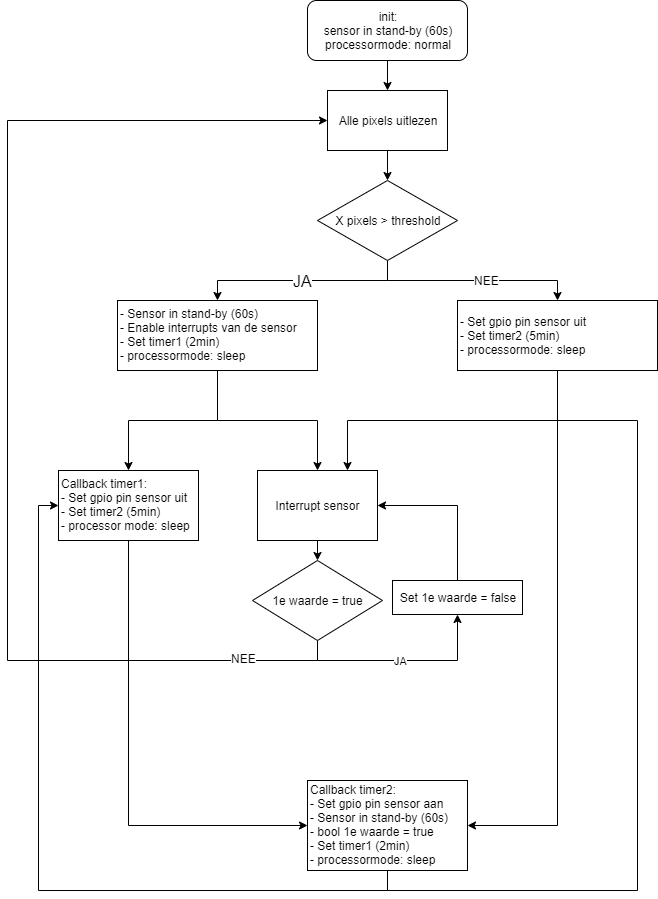
\includegraphics[scale=0.5]{flowchartcode.png}
	\caption{flowchart van de code}
	\label{fig:flowchart}
\end{figure}


\section{Power consumptie}

\subsection{Principe}
\paragraph{Sensor: }
Door de methode toe te passen die in besproken werd in section \ref{flowcode} wordt de power consumptie sterk verminderd. Wanneer er geen mensen aanwezig zijn, wordt het verbruik met 60 procent verminderd aangezien de sensor om de 5 minuten, 2 minuten aangezet wordt. Verder is het verbruik afhankelijk van hoe frequent er mensen in de wachtrij staan. In de berekeningen gaan we er van uit dat er enkel mensen aan het wachten zijn tussen 11u en 14u. In dit geval zal de sensor 3u per dag constant in stand-by staan aangezien er 3u lang mensen aanwezig zijn. Verder zal de sensor nog 21u 24 minuten per uur aanstaan om periodiek te kijken of er iemand aan het wachten is. Als we dit na rekenen bekomen we dat de sensor 11.4 uur in stand-by staat. Dit komt uit op een stroom verbruik van: 
\begin{equation}
	\frac{11.4 h\cdot 0.8 mAh}{24 h} = 0.38 mAh
\end{equation}

\paragraph{Processor: }

\subsection{Metingen}


\section{Besluit }



\end{document}
